\section*{Problem 1}

$R(t)$: balloon radius; $\rho_i$ and $\rho_o$: inside and outside densities.
The densities are constant, and the inlet-tube volume is negligible.
\[
Q=2.0\times10^{-3}\ \mathrm{m^3/s},\quad
\rho_i=1.30\ \mathrm{kg/m^3},\quad \rho_o=1.20\ \mathrm{kg/m^3},\quad
R_0=0.10\ \mathrm m,\quad R_c=0.15\ \mathrm m.
\]

\partlabel{(a)}
$\mathbf n$: outward unit normal; $\mathbf u_b$: control-surface velocity.
The control surface follows the membrane and cuts the inlet tube.
% Unit 2, Lecture 5 organized notes, PDF p.5, Eqs. (33)--(35).
\[
0=\frac{d}{dt}\int_{V_b(t)}\rho\,dV
  +\int_{S_b(t)}\rho(\mathbf u-\mathbf u_b)\cdot\mathbf n\,dA.
\]
At the membrane,
\[
\mathbf u\cdot\mathbf n=\mathbf u_b\cdot\mathbf n=\frac{dR}{dt}
\quad\Longrightarrow\quad
\rho_i(\mathbf u-\mathbf u_b)\cdot\mathbf n
=\rho_i\left(\frac{dR}{dt}-\frac{dR}{dt}\right)=0.
\]
With $Q$ evaluated at the inlet density $\rho_i$,
\begin{align*}
\frac{d}{dt}(\rho_i V_b)-\rho_i Q&=0,
& V_b&=\frac{4\pi}{3}R^3,\\
\rho_i4\pi R^2\frac{dR}{dt}&=\rho_i Q
&\Longrightarrow\quad
\boxed{\frac{dR}{dt}=\frac{Q}{4\pi R^2}}&.
\end{align*}

\partlabel{(b)}
\[
\left.\frac{dR}{dt}\right|_{R=0.15\,\mathrm m}
=\frac{2.0\times10^{-3}}{4\pi(0.15)^2}
=\boxed{7.07\times10^{-3}\ \mathrm{m/s}}.
\]

\partlabel{(c)}
\begin{gather*}
\frac{dV_b}{dt}=Q
\quad\Longrightarrow\quad
V_b(t)-V_b(0)=Qt,\\
\frac{4\pi}{3}\bigl[R^3(t)-R_0^3\bigr]=Qt
\quad\Longrightarrow\quad
R(t)=\left(R_0^3+\frac{3Qt}{4\pi}\right)^{1/3}.
\end{gather*}
Let $t_c$ be the time at which $R(t_c)=R_c$:
\[
t_c=\frac{4\pi(R_c^3-R_0^3)}{3Q}
=\frac{4\pi[(0.15)^3-(0.10)^3]}{3(2.0\times10^{-3})}
=\boxed{4.974\ \mathrm s}.
\]

\newpage
\partlabel{(d)}
$M(t)$ is the total gas mass inside the fixed sphere, including both gases.
\begin{align*}
V_c&=\frac{4\pi}{3}R_c^3,\qquad
V_{b,0}=\frac{4\pi}{3}R_0^3,\\
M(t)&=\rho_iV_b(t)+\rho_o[V_c-V_b(t)]\\
&=\rho_oV_c+(\rho_i-\rho_o)(V_{b,0}+Qt).
\end{align*}
\[
\boxed{M(t)=0.0173835\ \mathrm{kg}
+\left(2.00\times10^{-4}\ \mathrm{kg/s}\right)t,
\qquad 0\le t\le t_c.}
\]
\[
M(0)=17.3835\ \mathrm g,\qquad M(t_c)=\rho_iV_c=18.3783\ \mathrm g.
\]
\begin{center}
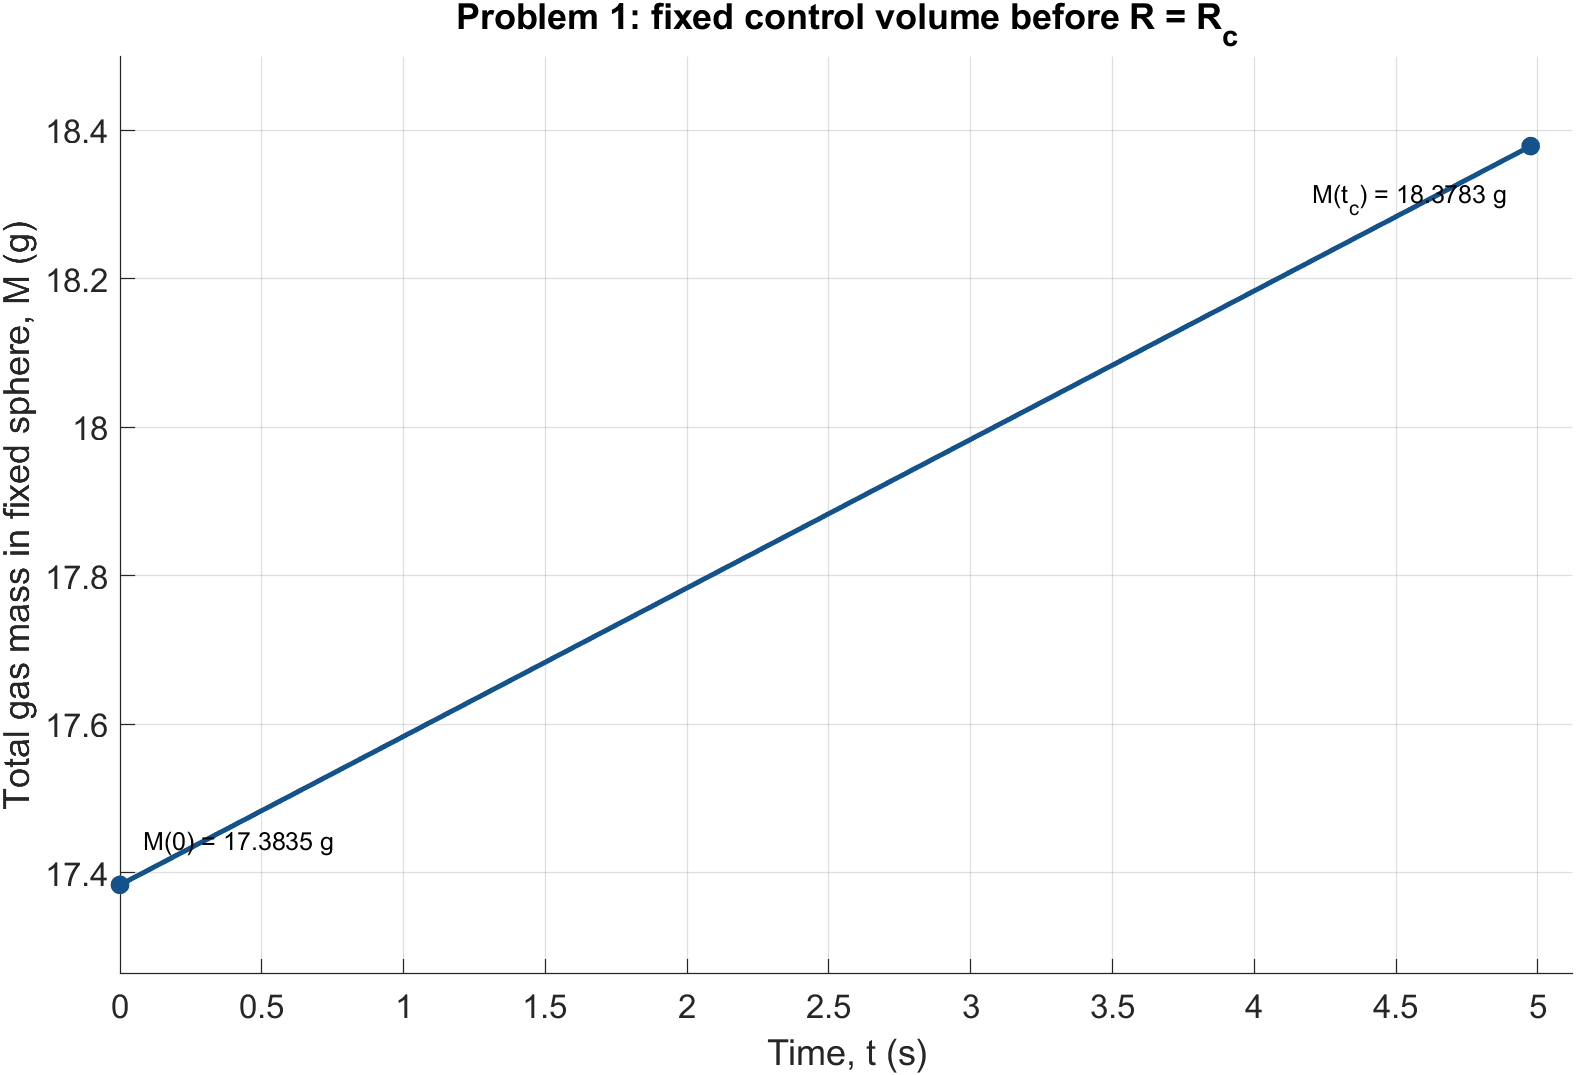
\includegraphics[width=0.58\linewidth]{figures/HW2_Problem1_Mass.png}
\end{center}

\partlabel{(e)}
For $R>R_c$, the fixed sphere contains only gas of density $\rho_i$.
Define the outward radial component and its surface average by
\[
u_r=\mathbf u\cdot\mathbf n,\qquad
\overline u_r=\frac{1}{4\pi R_c^2}\int_{S_c}u_r\,dA.
\]
% Unit 2, Lecture 5 organized notes, PDF p.5, Eq. (36).
\begin{gather*}
M=\rho_iV_c=\text{constant},\qquad
\frac{dM}{dt}+\rho_i4\pi R_c^2\overline u_r-\rho_iQ=0,\\
\boxed{\overline u_r=\frac{Q}{4\pi R_c^2}
=7.07\times10^{-3}\ \mathrm{m/s}\quad\text{(outward)}.}
\end{gather*}
The inlet is counted separately; its small opening area is neglected.

\partlabel{(f)}
\[
\begin{aligned}
\text{Moving balloon volume:}\quad
&\frac{d}{dt}(\rho_iV_b)=\rho_iQ,\\
\text{Fixed sphere, }R<R_c:\quad
&\frac{dM}{dt}=\rho_iQ-\rho_oQ=(\rho_i-\rho_o)Q,\\
\text{Fixed sphere, }R>R_c:\quad
&\frac{dM}{dt}=\rho_iQ-\rho_iQ=0.
\end{aligned}
\]
Both satisfy mass conservation. The moving membrane has zero relative mass
flux, whereas gas crosses the fixed spherical surface; the enclosed mass
therefore changes differently.
